\documentclass[aspectratio=1610]{beamer}
\usepackage{tikz}
\PassOptionsToPackage{height=1.2cm}{beamerouterthemesidebar}

% Theme
\usetheme{LMPS} % LMPS inspired


% packages 
\usecolortheme{default}
\usepackage{xcolor}
\usepackage{multicol}
\usepackage{multirow}
\newcommand\hmmax{0}
\newcommand\bmmax{0}
\usepackage{soul}

% My notations
\usepackage{MyNotations}





%%%%%%%%%%%%%%%%%%%%%% User commands %%%%%%%%%%%%%%%%%%%%%%
% To remove "Figure" from caption
\captionsetup{labelformat=empty,labelsep=none} 
\usefonttheme[onlymath]{serif}% Serif pour la police math

\usetikzlibrary{calc}
% https://tex.stackexchange.com/questions/601835/drawing-arrow-between-subfigures-in-scaleboxes

% To scale tikz figures from external files
\newcommand{\inputTikZ}[2]{%  
	\scalebox{#1}{\input{#2}}  
}

%% Data 
\title[Seminar ] %optional
{\bfseries \textcolor{BleuLMPS}{Towards an Optimal Multi-query Framework
		based on Model-order Reduction for
		Non-linear Dynamics}
}
\subtitle{\itshape\textcolor{BleuLMPS}{ Seminar}}
\author[A. Daby-S.] % (optional)
{\textbf{\textcolor{BleuLMPS}{A.~Daby-Seesaram}} \\[47pt] \textcolor{BleuLMPS!80}{Supervised by D.~N\'eron, A.~Fau and P.-\'E.~Charbonnel} }



\date[VLC 2023] % (optional)
{\textcolor{BleuLMPS!80}{29$^{\text{st}}$ of January 2024}}


\begin{document}
	%	
	{
		
		\setbeamertemplate{background} 
		{	\hspace*{\sidebarwidth}
			\hspace{-0.25cm}
			
			\includegraphics[width=\imagewidth]{Logos/LMPS/PipeZoomed2_light.png}
		}
		
		\frame{\titlepage} 
	}
	%---------------------------------------------------------
	
	
	\section{Introduction}
	

	\begin{frame}
		\frametitle{\textsc{Industrial context}}
		\framesubtitle{Structural elements} \vspace*{-17pt}
		\begin{figure}
			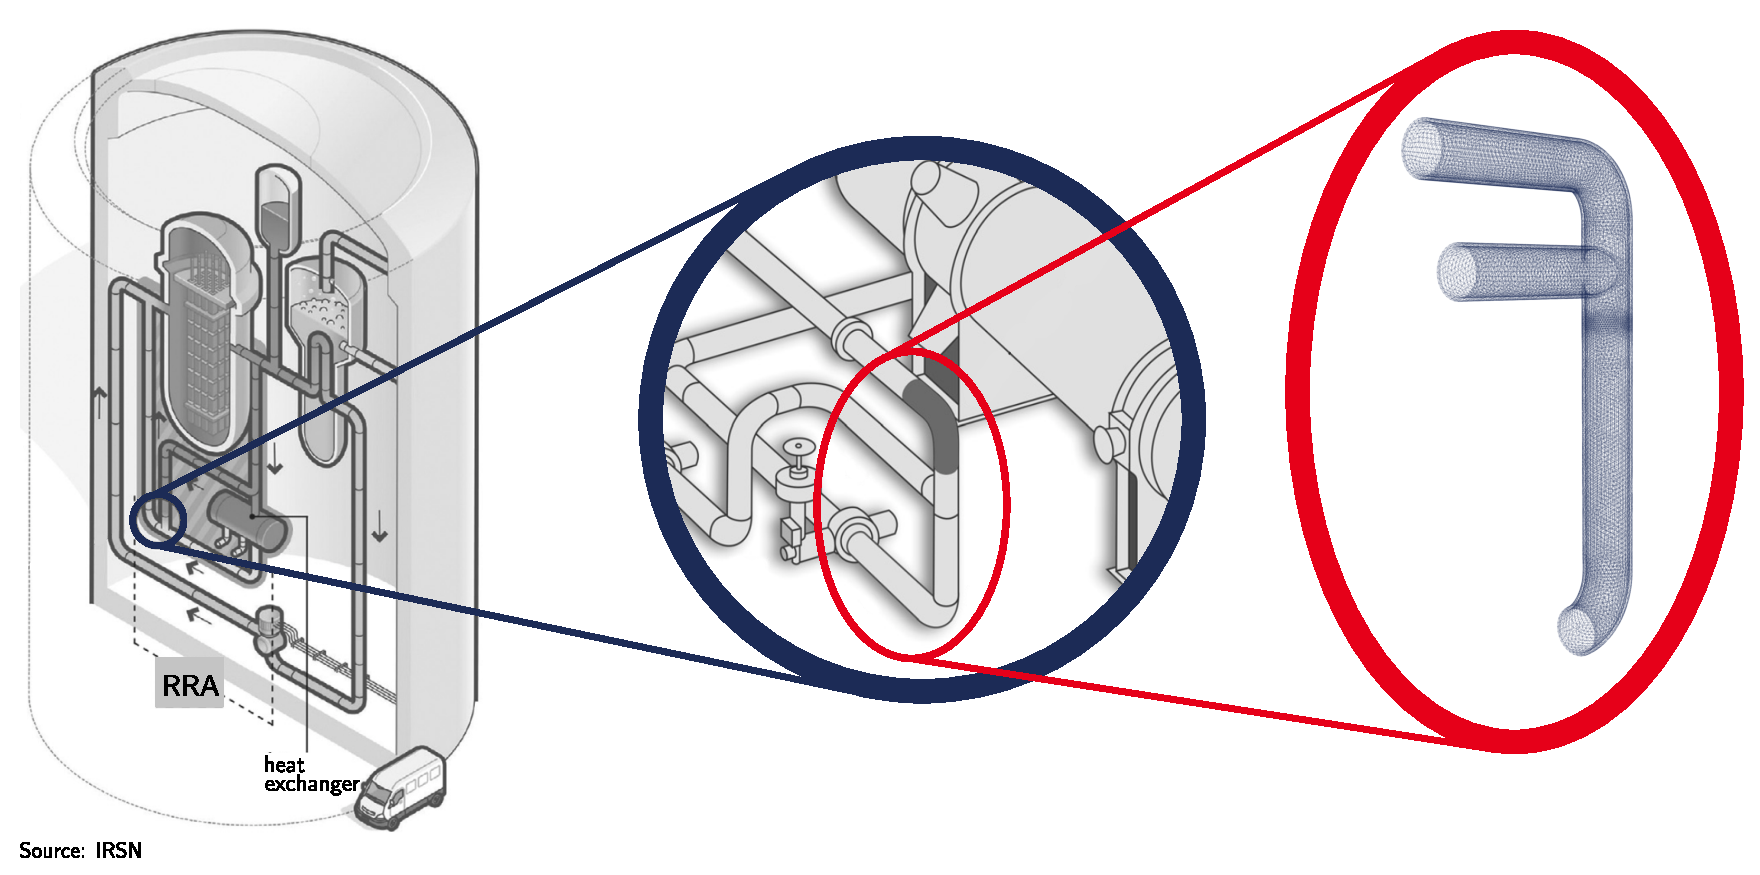
\includegraphics[width=0.85\linewidth]{Figures/Intro/RRA.eps}
		\end{figure}
		\onslide<2->{
			\begin{minipage}{0.55\linewidth}
				\begin{greenblockshadow}{Nominal operation}
					\begin{itemize}
						\item Piping component - Cooling system
						\begin{itemize}
							\item Thermal conditions: $20-\SI{180}{\celsius}$
							\item Ageing (thermal fatigue)
						\end{itemize}
					\end{itemize}
				\end{greenblockshadow}
		\end{minipage}}
		\hfill
		\onslide<3>{
			\begin{minipage}{0.43\linewidth}

				\begin{greenblockshadow}{Extreme conditions}
					\begin{itemize}
						\item Seismic hazard
						\begin{itemize}
							\item[\textcolor{BleuLMPS}{\faLightbulb}] Assessing the \textcolor{BleuLMPS}{\textbf{risk of failure}} \vspace{2pt}
						\end{itemize}
					\end{itemize}
				\end{greenblockshadow}
		\end{minipage}}
	\end{frame}
	
	\begin{frame}
		\frametitle{\textsc{Industrial context}}
		\framesubtitle{Variability of seismic loading}
		\begin{tikzpicture}[remember picture,overlay]
			\node[anchor=north west,inner sep=0] (imLeft) at ([xshift=2.5cm,yshift=-6cm]current page.north west) {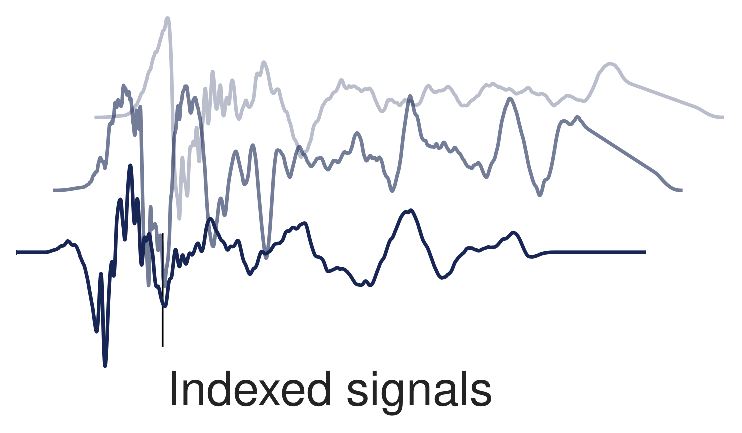
\includegraphics[width=0.4\linewidth]{Figures/Intro/Signals.eps}};
			\hphantom{text}
		\end{tikzpicture}
		\begin{minipage}{0.58\linewidth}
			\begin{greenblockshadow}{Account for the variability}
				\begin{itemize}
					\item Wide range of plausible earthquake signals ($\sim 1000$)
					\item Sort the signals by severity ($\alpha$)
					\item Compute a failure probability ($P_f$) for each severity level
				\end{itemize}
			\end{greenblockshadow}
		\end{minipage}
		\hfill
		\begin{minipage}{0.4\linewidth}
			\begin{figure}
				\centering
				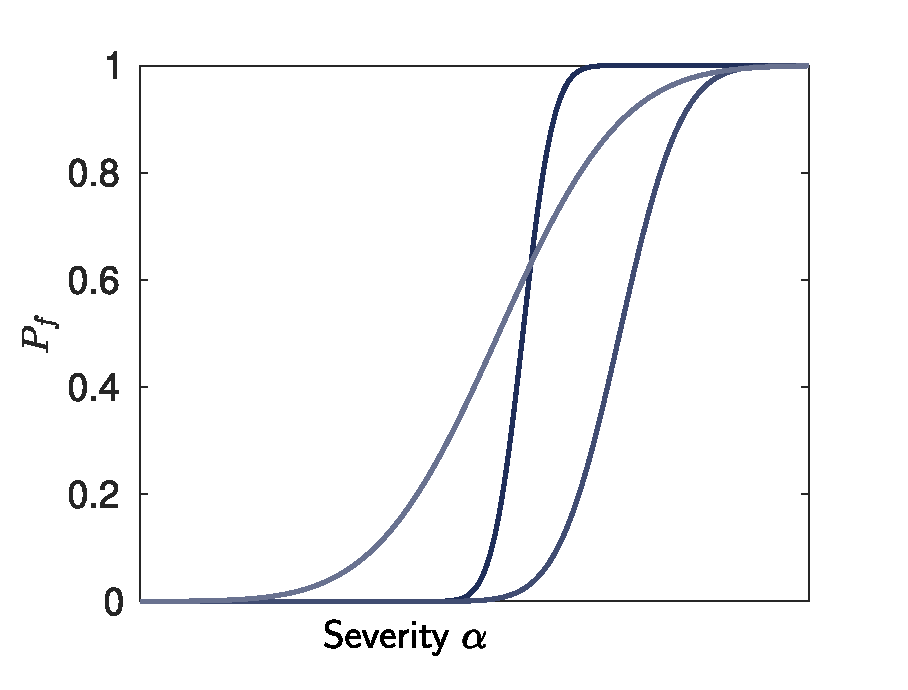
\includegraphics[width=\linewidth]{Figures/Intro/Fragility_4.eps}
			\end{figure}
		\end{minipage}
		\onslide<2>{
			\begin{orangeblockshadow}{In practice}
				\begin{itemize}
					\item Parametrised (lognormal) \citeperso{[Kennedy, et al., 1980]}
					\begin{itemize}
						\item Fewer computations 
						\item Bias in the probability prediction \citeperso{[Mandal, et al., 2016]}
					\end{itemize}
					\item Simplified mechanical model or high computational cost 
					\item[\faLock] Fine structural description combined with accounting for the ageing of the strucure
					\begin{itemize}
						\item Workpackage II of NARSIS Project
					\end{itemize}
				\end{itemize}
		\end{orangeblockshadow}}
	\end{frame}
	
	\begin{frame}
		\frametitle{\textsc{Industrial context}}
		\framesubtitle{Multi-query requirement \citeperso{[NARSIS WP2]}}
		
		\begin{overprint}
			\onslide<1>
			\begin{tikzpicture}[remember picture,overlay]
				\node[anchor=north west,inner sep=0] (imLeft) at ([xshift=1.8cm,yshift=-1.5cm]current page.north west) {\inputTikZ{0.5}{Figures/Tikz/Algo_Indus_ini_2.tex}};
			\end{tikzpicture}
			\onslide<2>
			\begin{tikzpicture}[remember picture,overlay]
				\node[anchor=north west,inner sep=0] (imLeft) at ([xshift=1.8cm,yshift=-1.5cm]current page.north west) {\inputTikZ{0.5}{Figures/Tikz/Algo_Indus_mid_2.tex}};
			\end{tikzpicture}
			\onslide<3>
			\begin{tikzpicture}[remember picture,overlay]
				\node[anchor=north west,inner sep=0] (imLeft) at ([xshift=1.8cm,yshift=-1.5cm]current page.north west) {\inputTikZ{0.5}{Figures/Tikz/Algo_Indus_2.tex}};
				\node[anchor=north east,inner sep=0] (imRight) at ([xshift=-0.2cm,yshift=-2.1cm]current page.north east) {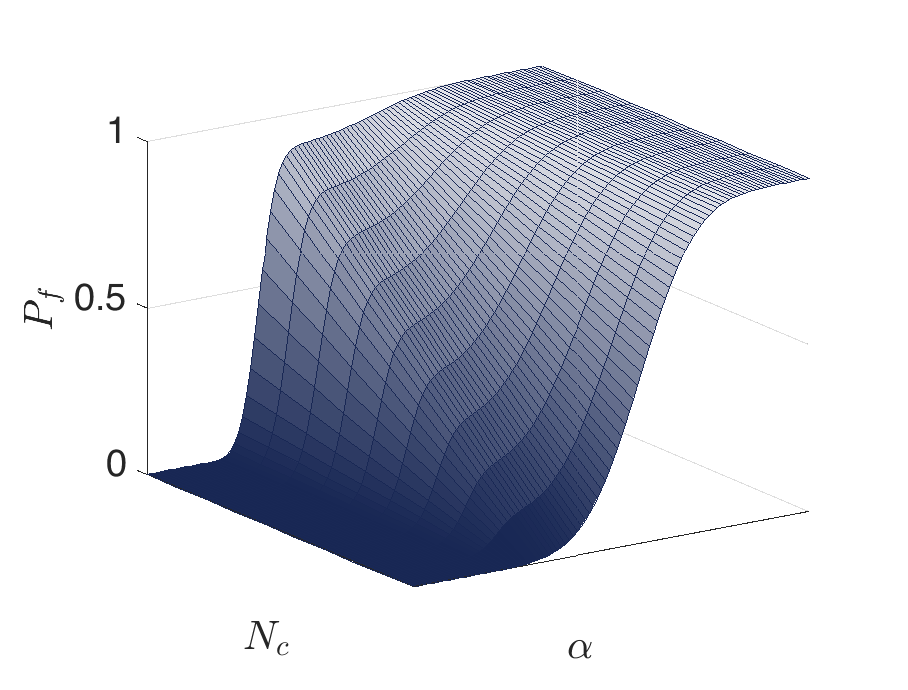
\includegraphics[width=0.4\linewidth]{Figures/Intro/Surface_fragility.eps}};
				\node[anchor=south west,inner sep=0] (ImSouth) at ([xshift=1.8cm,yshift=0.5cm]current page.south west) {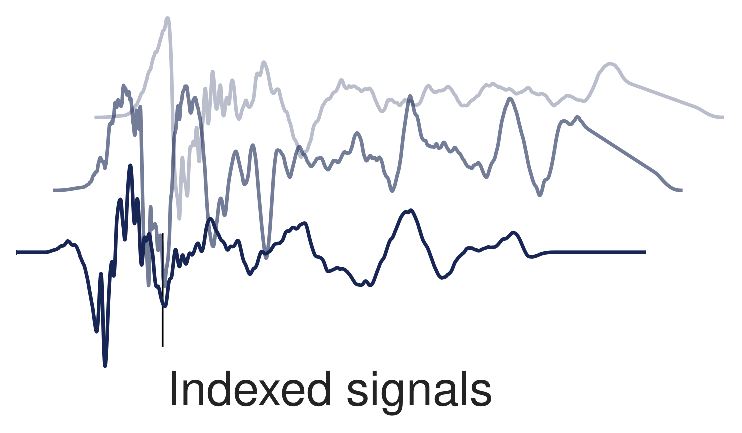
\includegraphics[height=2cm]{Figures/Intro/Signals.eps}};
				
				%		\draw[->,thick] (ImSouth) -- ($(C)!0.5!(Database)$);
				-		\draw[BleuLMPS,-{Stealth[scale = 1]},thick] (ImSouth) -- ++(-0.8,1.9); 
				-		\draw[BleuLMPS,{Stealth[scale = 1]}-,thick] (imRight.west) -- ++(-0.8,0); 
			\end{tikzpicture}
			\begin{minipage}{0.3\linewidth}
				\vfill
				\vphantom{text}
			\end{minipage}
			\hfill
			\begin{minipage}{0.6\linewidth}
				\begin{minipage}[0.5\textheight]{\textwidth}
					\vphantom{\begin{greenblockshadow}{\faCogs}
							\begin{itemize}
								\item Ageing assessment
								\begin{itemize}
									\item Thermal Fatigue
								\end{itemize}
								\item Non-parametrised signals
								\begin{itemize}
									\item Multiple queries to the solver
								\end{itemize}
								\item Failure probability $P_f$
								\begin{itemize}
									\item Function of a severity parameter $\alpha$
								\end{itemize}
							\end{itemize}
							\vspace{40pt}
					\end{greenblockshadow}}
				\end{minipage}
				\vfill
				\begin{minipage}[0.5\textheight]{\textwidth}
					\begin{greenblockshadow}{\faCogs~ Failure probability under seismic loading}
						\begin{itemize}
							\item Non-parametrised signals $\left[\SI{0}{Hz},\SI{30}{Hz}\right]$
							\begin{itemize}
								\item Multiple queries to the solver
							\end{itemize}
							\item Fragility surface
							\begin{itemize}
								\item Additional dimension $N_c$
							\end{itemize}
						\end{itemize}
					\end{greenblockshadow}
				\end{minipage}
			\end{minipage}
		\end{overprint}
		
		
		
	\end{frame}
	
	\begin{frame}
		\frametitle{\textsc{Outline}}
		\vspace{-1.5cm}
		\begin{itemize}
			\item[\faLightbulb] 	\textbf{How to efficiently compute fragility surfaces? }
		\end{itemize}
		\vspace{1.5cm}
		\begin{overprint}
			\onslide<1>
			\begin{tikzpicture}[remember picture,overlay]
				\node[anchor=north west,inner sep=0] (imLeft) at ([xshift=1.5cm,yshift=-3cm]current page.north west) {\inputTikZ{0.5}{Figures/Tikz/Algo_Indus_solver_2.tex}};
				\hphantom{text}
			\end{tikzpicture}
			\onslide<2>
			\begin{tikzpicture}[remember picture,overlay]
				\node[anchor=north west,inner sep=0] (imLeft) at ([xshift=1.5cm,yshift=-3cm]current page.north west) {\inputTikZ{0.5}{Figures/Tikz/Algo_Indus_MultiQuery_3.tex}};
			\end{tikzpicture}
			\onslide<3>
			\begin{tikzpicture}[remember picture,overlay]
				\node[anchor=north west,inner sep=0] (imLeft) at ([xshift=1.5cm,yshift=-3cm]current page.north west) {\inputTikZ{0.5}{Figures/Tikz/Algo_Indus_MultiFidelity_2.tex}};
			\end{tikzpicture}
		\end{overprint}
		
		\begin{minipage}{0.56\linewidth}
			\vphantom{text}
		\end{minipage}
		\hfill
		\begin{minipage}{0.42\linewidth}
			\begin{itemize}
				\setlength\itemsep{1em}
				\item[\textcolor{BleuLMPS}{\textbf{I} - }]\textcolor{BleuLMPS}{\textbf{Efficient solver}}

				\onslide<2->{
					\item[\textcolor{RougeCEA!80!black}{\textbf{II} - }]\textcolor{RougeCEA!80!black}{\textbf{Multi-query framework}}

				}
				\onslide<3>{
					\item[\textcolor{Greendaby}{\textbf{III} - }]\textcolor{Greendaby}{\textbf{Application to classification}}\!

				}
			\end{itemize}
		\end{minipage}
		
		
	\end{frame}
	
	\section{Efficient solver}
	
	\begin{frame}
		\frametitle{\textsc{Hybrid method}}
		\framesubtitle{Space-frequency reduced-order model method}
		\begin{center}
			{\Huge \textcolor{BleuLMPS}{I - Efficient solver}}\\[20PT]
			\begin{minipage}{0.4\linewidth}
				\begin{itemize}
					\item[\textcolor{BleuLMPS!80}{\faMapSigns}] \textcolor{BleuLMPS!80}{Requirements:} 				
					\begin{itemize}
						\item \textcolor{BleuLMPS!60}{Low-frequency dynamics}
						\item \textcolor{BleuLMPS!60}{Ductile damage}
						\item \textcolor{BleuLMPS!60}{Low computational cost}
					\end{itemize}
				\end{itemize}
			\end{minipage}
		\end{center}
	\end{frame}
	
	
	\subsection{ROM}
	\begin{frame}
		\frametitle{\textsc{Reduced-order model}}
		\framesubtitle{Low-rank approximation of the solution }
		\begin{minipage}{0.48\linewidth}
			\begin{greenblockshadow}{Full-order discretised model}
				\begin{itemize}
					\item $N$ spatial shape functions
					\begin{itemize}
						\item Span a finite spatial space of dimension $N$
					\end{itemize}
					\item Requires computing $N$ associated temporal functions
				\end{itemize}
			\end{greenblockshadow}
		\end{minipage}
		\hfill
		\begin{minipage}{0.48\linewidth}
			\begin{greenblockshadow}{Reduced-order model}
				\begin{itemize}
					\item $m \ll N$ spatial modes
					\begin{itemize}
						\item Similar to global shape functions
						\item[\faLightbulb] Span a smaller space
					\end{itemize}
					\item[\faCogs] Galerkin projection 
				\end{itemize}
				\vspace{1pt}
			\end{greenblockshadow}
		\end{minipage}
		\vfill
		\begin{orangeblockshadow}{\faCogs \quad Finding the reduced-order basis}
			
			\begin{itemize}
				\item Linear Normal Modes (eigenmodes of the structure) {\footnotesize\citeperso{[Hansteen \& Bell, 1979]}}
				\begin{itemize}
					\item Do not account for the loading and behaviour specifics
				\end{itemize}
				\item Proper Orthogonal Decomposition {\footnotesize\citeperso{[Chatterjee, 2000],[Radermacher \& Reese, 2013]}}
				\begin{itemize}
					\item Require wise selection of the snapshots and \emph{a priori} costly computations 
				\end{itemize}
				\item Reduced basis method {\footnotesize\citeperso{[Maday \& Rønquist, 2002]}} with EIM {\footnotesize\citeperso{[Barrault et al., 2004]}}
				\begin{itemize}
					\item Rely on prior expensive computations
				\end{itemize}
			\end{itemize}
		\end{orangeblockshadow}
	\end{frame}
	
	\begin{frame}
		\frametitle{\textsc{Reduced-order model}}
		\framesubtitle{Proper Generalised Decomposition (PGD)}		
		
		\begin{minipage}{0.53\linewidth}
			

			\begin{greenblockshadow}{Choice of separation of variables}
				\begin{overprint}
					\vspace{7pt}
					Extracoordinates {\footnotesize\citeperso{[Chinesta et al., 2011]}}
					\begin{itemize}
						\item \small{$\displaystyle\vect{u}(\textcolor{LightBleuLMPS}{\vect{x}},\textcolor{RougeCEA}{\omega},\textcolor{VertLMPS}{\vect{\mu}}) = \sum\limits_{i=1}^m \textcolor{LightBleuLMPS}{\overline{\vect{u}}^i(\vect{x})} ~\textcolor{RougeCEA}{\lambda^i_{\omega}(\omega)}~\textcolor{VertLMPS}{\prod_{j=1}^{n}M_j^i(\vect{\mu})}$} 
						\begin{itemize}
							\item Expression of the full parametrised solution
							\item Single computation
							\item Problem dependent
						\end{itemize}
					\end{itemize}
					\onslide<2>
					\vspace{8pt}
					Out of the decomposition {\footnotesize\citeperso{[Ladevèze, 1985]}}
					\begin{itemize}
						\item  $\vect{u}_{\textcolor{VertLMPS}{\mu}}(\textcolor{LightBleuLMPS}{\vect{x}},\textcolor{RougeCEA}{\omega}) = \sum\limits_{i=1}^m \textcolor{LightBleuLMPS}{\overline{\vect{u}}^i(\vect{x})} ~\textcolor{RougeCEA}{\lambda^i_{\omega}(\omega)}$ 
						\begin{itemize}
							\item More versatile {\footnotesize\citeperso{[Scanff et al., 2022]}}
							\item Suited to non-parametrised problems
						\end{itemize}
					\end{itemize}
				\end{overprint}
			\end{greenblockshadow}
			
			
			
		\end{minipage}
		\hfill
		\begin{minipage}{0.45\linewidth}
			\begin{overprint}
				\vspace{7pt}
				\begin{figure}
					\centering
					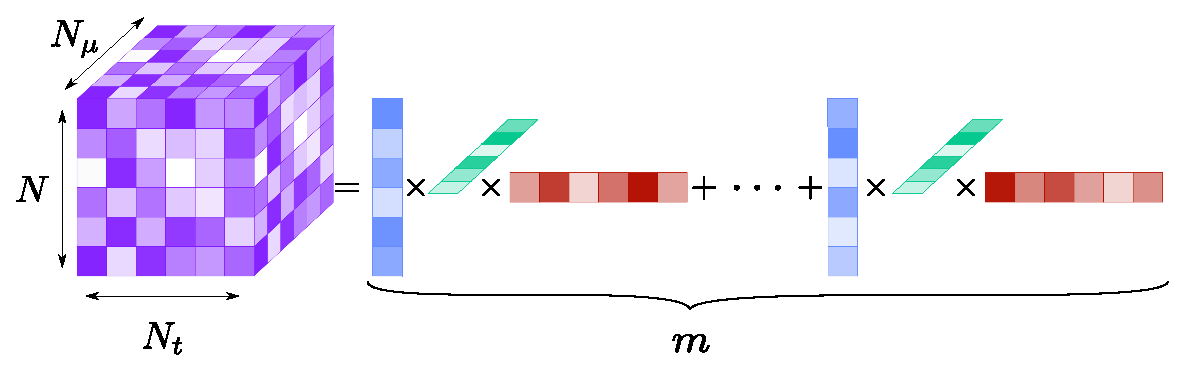
\includegraphics[width=\linewidth]{Figures/PGD_Method_Matrix_3D.eps}
				\end{figure}
				\vfill \vspace{30pt}
				\onslide<2>
				\begin{figure}
					\centering
					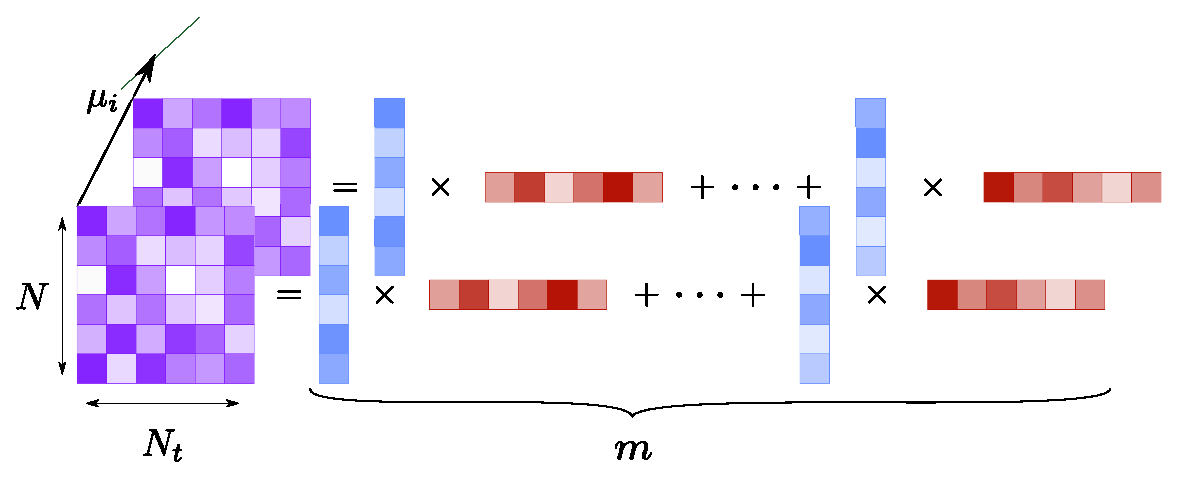
\includegraphics[width=\linewidth]{Figures/PGD_Method_Matrix_2D_2.eps}
				\end{figure}
			\end{overprint}
		\end{minipage}
	\end{frame}
	
	
	
	
	
	\begin{frame}
		\frametitle{\textsc{Reduced-order model}}
		\framesubtitle{Proper Generalised Decomposition (PGD)}		
		
		\begin{minipage}{0.53\linewidth}
			\begin{greenblockshadow}{PGD}
				\vspace*{8pt}
				\begin{itemize}
					\item  $\vect{u}(\textcolor{LightBleuLMPS}{\vect{x}},\textcolor{RougeCEA}{\omega}) = \sum\limits_{i=1}^m \textcolor{LightBleuLMPS}{\overline{\vect{u}}^i(\vect{x})} ~\textcolor{RougeCEA}{\lambda^i_{\omega}(\omega)}$
					\begin{itemize}
						\item Spatial modes $\textcolor{LightBleuLMPS}{\overline{\vect{u}}^i(\vect{x})}$
						\item Frequency modes $\textcolor{RougeCEA}{\lambda^i_{\omega}(\omega)}$
					\end{itemize}
					\item For a given basis {\footnotesize$\left\{\overline{\vect{u}}^i(\vect{x})\right\}_{i \in \llbracket 1,m\rrbracket}$}
					\begin{itemize}
						\item Update the associated frequency functions
						\begin{itemize}
							\item Similar to POD
						\end{itemize}
					\end{itemize}
					\item Add new modes on the fly
					\begin{itemize}
						\item Generate modes targeted for the current problem
						\item Greedy algorithm
					\end{itemize}
					\vspace*{8pt}
				\end{itemize}
			\end{greenblockshadow}
		\end{minipage}
		\hfill
		\begin{minipage}{0.45\linewidth}
			\vspace{38pt}
			\begin{figure}
				\centering
				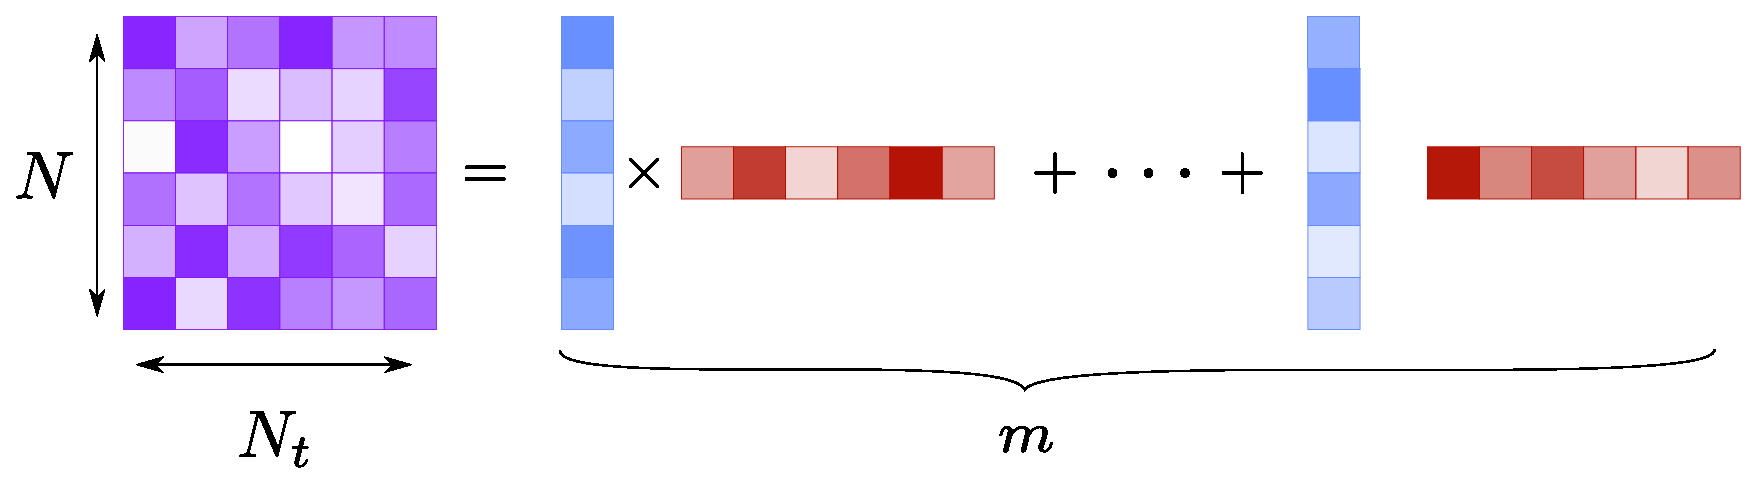
\includegraphics[width=\linewidth]{Figures/PGD_Method_Matrix_2.eps}
			\end{figure}
			\vspace{10pt}
			\begin{orangeblockshadow}{\faCogs ~ Requirements}
				\begin{itemize}
					\item Linear equations
					\begin{itemize}
						\item Linearisation strategy for non-linear problems
					\end{itemize}
					\item Global computations in space and time
					\begin{itemize}
						\item Non-incremental scheme
					\end{itemize}
				\end{itemize}
			\end{orangeblockshadow}
		\end{minipage}
		
	\end{frame}
	
	
		
	\end{document}
	
	
	
	
	
